\documentclass{article}
\usepackage{tikz,lipsum,lmodern}
\usepackage[english]{babel}
\usepackage[most]{tcolorbox}
\usepackage[paperheight=10.75in,paperwidth=7.25in,margin=1in,heightrounded]{geometry}
\usepackage{graphicx}
\usepackage{blindtext}
\usepackage{ragged2e}
\usepackage{needspace}
\usepackage[space]{grffile}
\usepackage[utf8]{inputenc}
\usepackage[export]{adjustbox}
\usepackage{hyperref}
\usepackage{placeins}

\hypersetup{
    colorlinks,
    citecolor=black,
    filecolor=black,
    linkcolor=black,
    urlcolor=black
}
\usepackage{fancyhdr}
\pagestyle{fancy}
\fancyhf{}
\rhead{\rightmark}
\chead{\thepart}
\lhead{\nouppercase{\leftmark}}
\cfoot{\thepage}
\graphicspath{{"./img/"}}


\newcommand{\lbl}[1]{(see image \ref{#1}, p. \pageref{#1}, \nameref{#1})}

\title{%
Neural Networks \\
\large Deep Learning}

\author{Silas Hoffmann, inf103088}
\date{\today}


\begin{document}
\maketitle

\vspace{0.5cm}
\tableofcontents
\vspace{0.5cm}

\section{Introduction}
Notes for the introduction to neural networks presented by \textbf{3blue1brown}. Watch the whole series here: \underline{todo paste link}. This series describes the strategy to recognize handwritten numbers.

\clearpage

\section{Chapter 1 - But what is a neural network?}


\subsection{Structure}

\FloatBarrier

\begin{figure}[h]
\centering
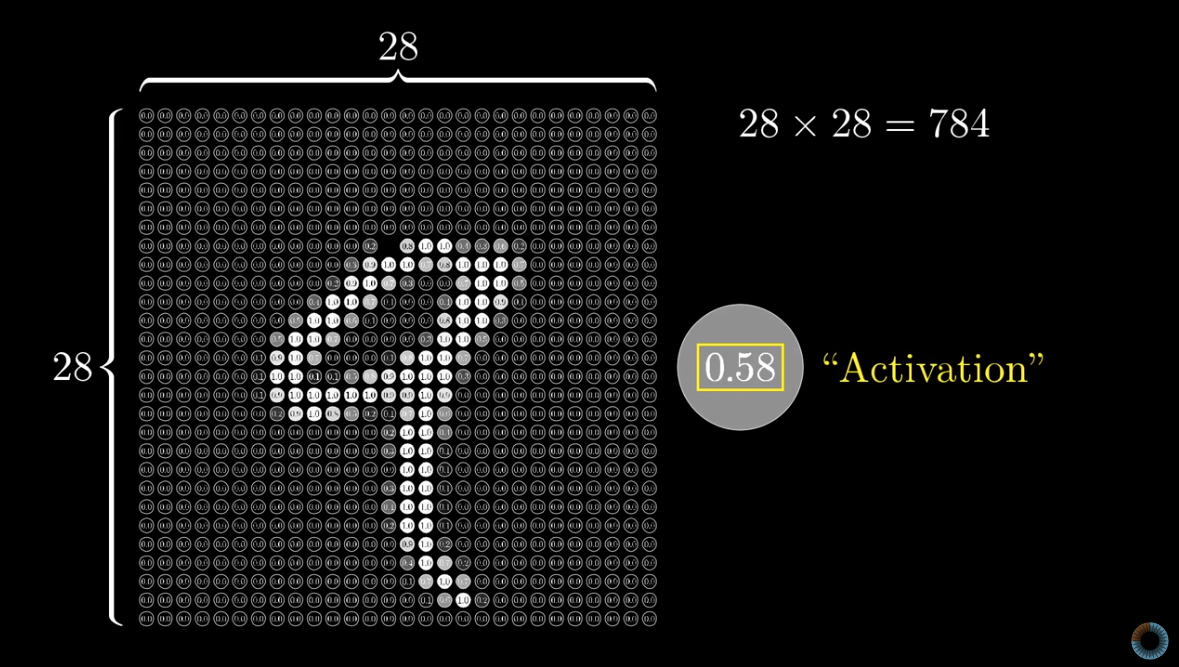
\includegraphics[max width=.9\textwidth]{ai_1.png}
\caption{Image interpreted as first layer of neural network}
\label{ai_1}
\end{figure}

Each pixel from the image is represented by a so called \textit{neuron} \lbl{ai_1}. These neurons possess a value called \textbf{Activiation} which contains a float between 0 and 1. This value specifies the brightness of this the particular pixel. This activation value also can be interpreted as how \textit{light up} this particular neuron actually is, 1 meaning 100 \% in this context.



\end{document}

